\chapter{النمو الخضري للنبات: المرستيمات والنمو}\label{ch:b2:plant-meristems}

بلوطة كانت بادرةً يوم بُنيت الكاتدرائية لا تزال
تضيف حلقة \omterm{def:b2:plant-meristems:wood}{خشب} كل سنة، ولا تزال تفتح أوراقًا جديدة كل
ربيع، ولا تزال تدفع أطراف جذور جديدة في التربة. ولا حيوان يفعل
هذا؛ فالحصان يكف عن النمو في الرابعة. والفرق أن النبات
يحتفظ، عند طرف كل فرع وكل جذر وفي أسطوانة
رقيقة داخل كل جذع، بجمهرات صغيرة من خلايا جنينية
--- هي \emph{المرستيمات} --- لا تكف عن الانقسام أبدًا، وتبني
جسم النبات خارجًا وصاعدًا ما دام حيًا. ينظر
هذا الفصل في تنظيم المرستيمين القميين والتحكم فيهما،
وفي كيف تنمو خلية نباتية، وكيف تقرر الهرمونات شكل
فرع، وكيف يثخن جذع.

\section{المرستيمات}

\begin{definition}[المرستيمات ونمطا النمو]\label{def:b2:plant-meristems:meristem}
\index{مرستيم}\index{مرستيم قمي للفرع}\index{مرستيم قمي للجذر}\index{كامبيوم}
\emph{المرستيم} جمهرة من خلايا صغيرة غير متمايزة
منقسمة تبقى طوال حياة النبات وتشتق
منها أنسجته كلها. أما \emph{المرستيم القمي للفرع} (SAM)
فعند طرف كل فرع يصنع الأوراق والساق، وفي الموسم، الأزهار؛
و\emph{المرستيم القمي للجذر} (RAM) خلف كل طرف جذر يصنع
الجذر؛ وهما معًا يقودان \emph{النمو الأولي}، أي استطالة
النبات. أما \emph{المرستيمات الجانبية} --- وهي \emph{\omterm{def:b2:plant-meristems:wood}{الكامبيوم
الوعائي}} و\emph{كامبيوم الفلين}، وهما أسطوانتان رقيقتان داخل السوق
والجذور --- فتقود \emph{النمو الثانوي}، أي التثخن الذي
يصنع \omterm{def:b2:plant-meristems:wood}{الخشب} \omterm{def:b2:plant-meristems:wood}{والقلف}. فنمو النبات إذن \emph{غير محدد}:
إذ تستطيع المرستيمات الاستمرار بلا نهاية، والنبات كائن
معياري، يكرر وحدة ورقة--عقدة--سلامية--برعم ما دامت
الظروف تسمح. وكل برعم إبطي مرستيم قمي ساكن، فيحمل النبات
آلاف نقاط النمو الاحتياطية.
\end{definition}

\begin{proposition}[قمة الفرع]\label{prop:b2:plant-meristems:sam}
\index{ترتيب الأوراق}\index{بدائية الورقة}\index{الفترة الورقية}
\omterm{def:b2:plant-meristems:meristem}{المرستيم القمي للفرع} قبة عرضها عُشر مليمتر، من بضع مئات
من الخلايا. وطبقته الخارجية أو طبقتاه (\emph{الغلالة}) لا تنقسم إلا
في مستوي السطح وتعطي البشرة؛ أما الكتلة تحتها
(\emph{الجسم}) فتنقسم في كل المستويات. وعند القمة تغذي
\emph{منطقة مركزية} من خلايا جذعية بطيئة الانقسام
\emph{منطقةً محيطية} من خلايا أسرع انقسامًا، تنشأ فيها \emph{بدائيات
الأوراق} نتوءات على فترات زمنية منتظمة (هي
\emph{\omterm{prop:b2:plant-meristems:sam}{الفترة الورقية}}، من ساعات إلى أيام) وبزوايا منتظمة حول
القبة (هو \emph{\omterm{prop:b2:plant-meristems:sam}{ترتيب الأوراق}}: متقابل، أو سواري، أو حلزوني عند
الزاوية الذهبية \qty{137.5}{\degree}، التي تضع كل ورقة جديدة في
أوسع فجوة تتركها البقية). وتحت ذلك تصنع \emph{منطقة ضلعية}
اللبَّ وتطيل الساق. وتتكون البدائية حيث يتراكم
هرمون الأوكسين في الطبقة السطحية، وهي إذ تنمو تنزح
الأوكسين من جوارها، ولهذا تنشأ البدائية التالية
أبعد ما يمكن عنها: فالنميط ذاتي التنظيم.
\end{proposition}

\begin{omfigure}
\begin{tikzpicture}[every node/.style={font=\scriptsize}]
  % dome
  \draw[thick, fill=omExo!12] (-2.2,0) .. controls (-2.2,1.6) and (-0.8,2.6) .. (0,2.6) .. controls (0.8,2.6) and (2.2,1.6) .. (2.2,0) -- (2.2,-1.4) -- (-2.2,-1.4) -- cycle;
  % tunica layers
  \draw[thick, omDef] (-2.2,0) .. controls (-2.2,1.5) and (-0.8,2.45) .. (0,2.45) .. controls (0.8,2.45) and (2.2,1.5) .. (2.2,0);
  \draw[thick, omDef] (-2.05,0) .. controls (-2.05,1.35) and (-0.75,2.3) .. (0,2.3) .. controls (0.75,2.3) and (2.05,1.35) .. (2.05,0);
  % zones
  \draw[thick, dashed, omThm, fill=omThm!15] (0,1.75) ellipse (0.6 and 0.55);
  \draw[thick, dashed, omProp] (0,0.9) ellipse (1.6 and 1.35);
  \draw[thick, dashed, omExo!70!black] (-0.9,-0.9) rectangle (0.9,-0.1);
  % primordia
  \draw[thick, fill=omExo!40] (-2.2,0.4) .. controls (-2.5,1.4) and (-1.6,1.9) .. (-1.55,1.3) .. controls (-1.5,0.9) and (-1.9,0.6) .. (-2.2,0.4);
  \draw[thick, fill=omExo!40] (2.2,0.2) .. controls (2.7,1.0) and (2.1,1.5) .. (1.75,1.1) .. controls (1.6,0.8) and (1.9,0.5) .. (2.2,0.2);
  % labels
  \draw (0.4,2.1) -- (3.2,2.6) node[right, align=left] {منطقة مركزية:\\خلايا جذعية بطيئة الانقسام};
  \draw (1.3,0.5) -- (3.2,1.4) node[right, align=left] {منطقة محيطية:\\انقسام سريع، وبدائيات أوراق};
  \draw (0.6,-0.5) -- (3.2,0.0) node[right, align=left] {منطقة ضلعية: اللبّ،\\واستطالة الساق};
  \draw (-1.7,1.5) -- (-3.0,2.4) node[left, align=right] {بدائية\\ورقة};
  \draw (-1.2,2.05) -- (-3.0,1.2) node[left, align=right] {الغلالة: انقسامات\\سطحية فقط};
  \draw (2.2,0.7) -- (3.2,-1.0) node[right, align=left] {البدائية التالية،\\على \qty{137.5}{\degree} دورانًا};
\end{tikzpicture}

{\small \omterm{def:b2:plant-meristems:meristem}{المرستيم القمي للفرع} في مقطع: غلالة من طبقة أو طبقتين
سطحيتين فوق جسم، ومنطقة مركزية من خلايا جذعية عند
القمة، ومنطقة محيطية تبرز فيها بدائيات الأوراق، ومنطقة
ضلعية تحتها.}
\end{omfigure}

\begin{omfigure}
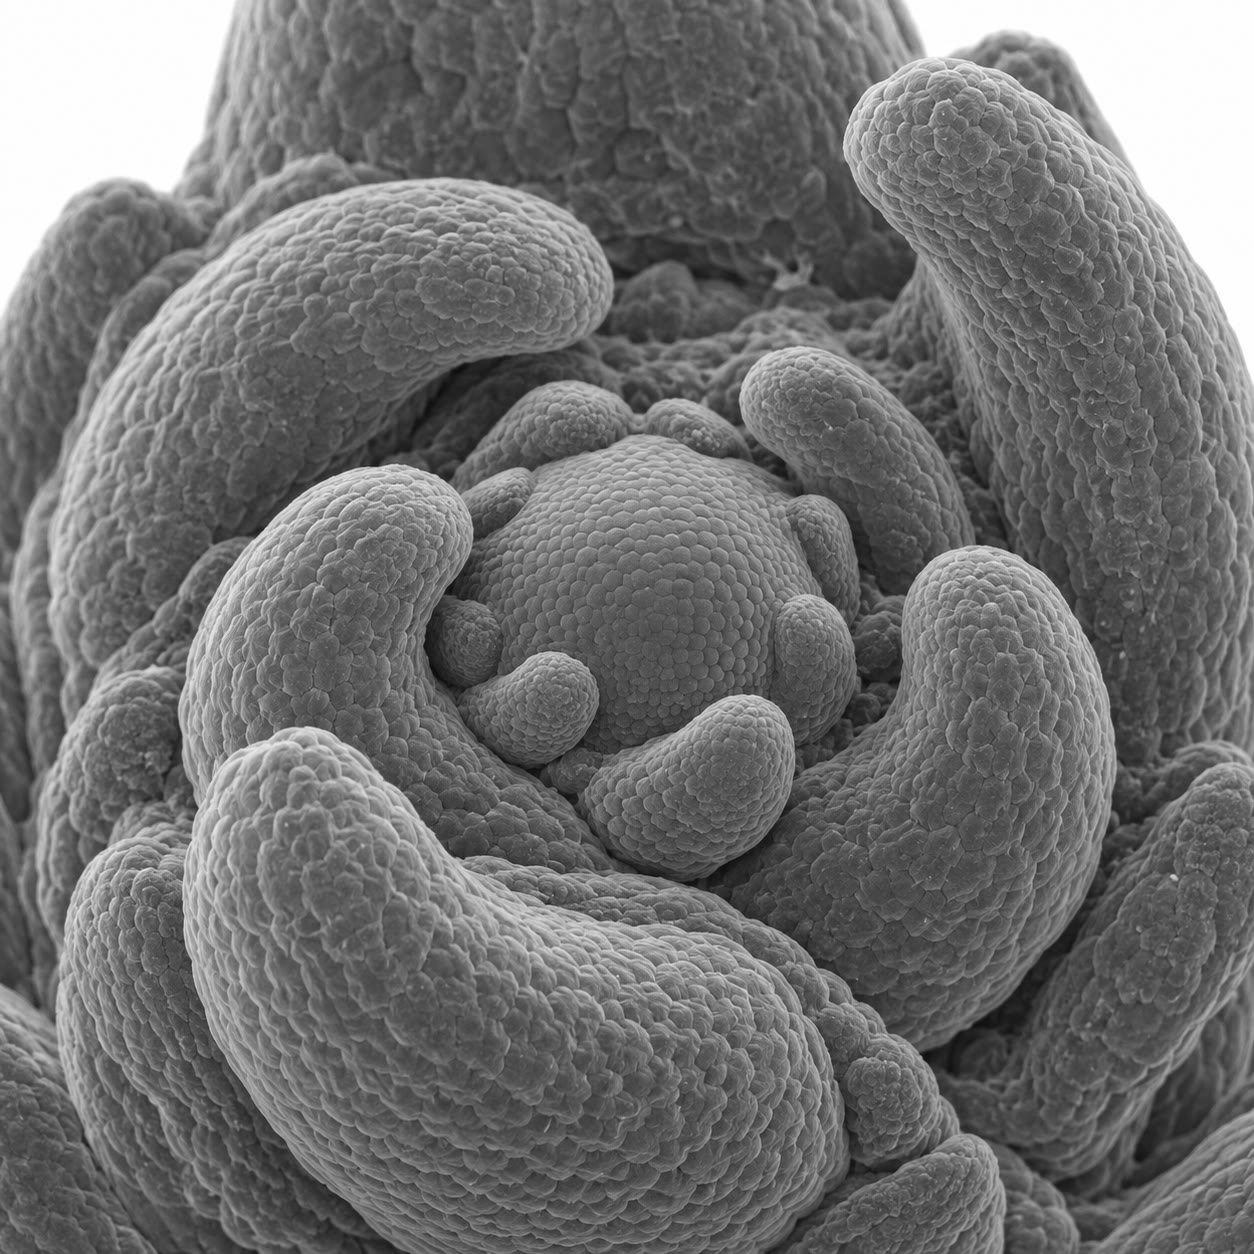
\includegraphics[width=0.44\linewidth]{images/book4/ai/b4-13-shoot-apex-sem.jpg}

{\small قمة فرع تحت المجهر الإلكتروني الماسح: قبة
\omterm{def:b2:plant-meristems:meristem}{المرستيم} الملساء وحلزون بدائيات الأوراق حولها،
وكل جديدة موضوعة في أوسع فجوة.}
\end{omfigure}

\begin{proposition}[إبقاء الخلايا الجذعية: حلقة تغذية راجعة]\label{prop:b2:plant-meristems:wus}
\index{WUSCHEL}\index{CLAVATA}\index{تغذية راجعة سالبة!المرستيم}
يُبقى قياس مخزون الخلايا الجذعية ثابتًا بحلقة بين
مورّثتين. فالخلايا تحت المنطقة المركزية مباشرة تعبّر عن
\omterm{prop:b2:cell-differentiation:transcriptional}{عامل الاستنساخ} \emph{WUSCHEL} (WUS)، وينتقل ناتجه صاعدًا
إلى الخلايا فوقه فيبقيها خلايا جذعية؛ وتفرز الخلايا
الجذعية بدورها ببتيدًا صغيرًا هو \emph{CLAVATA3} (CLV3)،
ينتشر نازلًا، ويرتبط بمستقبل كيناز (CLV1) في الخلايا المعبّرة
عن WUS فيكبت WUS. فخلايا جذعية أكثر تعني CLV3 أكثر وWUS أقل
وخلايا جذعية أقل؛ وخلايا جذعية أقل تعني CLV3 أقل وWUS أكثر وخلايا
جذعية أكثر. فالمخزون إذن مقدار منظَّم، كموجهتي الغدد
التناسلية في \cref{ch:b2:reproductive-hormones}، والمنطق نفسه ---
أي إشارة من الجمهرة المنظَّمة تكبت العامل
الذي يصنعها --- يحكم \omterm{def:b2:plant-meristems:meristem}{مرستيم} الجذر أيضًا.
\end{proposition}
\begin{proof}[شواهد]
طافرات \emph{clavata} في الأرابيدوبسيس (كلارك، وميروفيتز، في التسعينيات) لها
مرستيمات تنتفخ إلى أضعاف القياس السوي، بأوراق زائدة
وأعضاء زهرية زائدة وسوق مضفورة (مفلطحة شبيهة بالشريط):
فالكابح ذهب. أما طافرات \emph{wuschel} فتصنع مرستيمًا
يتوقف بعد أوراق قليلة ثم يكوّن مرستيمات جديدة يتوقف كل منها
بدوره: فالمسرّع ذهب. وفي الطافرة المضاعفة يسود \omterm{def:b2:meiosis-heredity:vocabulary}{النمط الظاهري}
\emph{wuschel}، فيقع WUS تحت CLV في المسار؛
وببتيد CLV3 المطبَّق على قمة برية يكبت WUS في غضون
ساعات.
\end{proof}

\begin{proposition}[قمة الجذر]\label{prop:b2:plant-meristems:ram}
\index{قلنسوة الجذر}\index{المركز الساكن}\index{منطقة الاستطالة}\index{شعرة جذرية}
ينمو الجذر من \omterm{def:b2:plant-meristems:meristem}{مرستيم} محتمٍ خلف \emph{قلنسوة جذر}
تُسلخ خلاياها مع دفع الطرف في التربة وهي
تفرز مخاطًا مزلقًا وتستشعر الجاذبية (بحبيبات نشاء
تستقر في خلاياها). وفي مركز \omterm{def:b2:plant-meristems:meristem}{المرستيم} لا ينقسم
\emph{مركز ساكن} من بضع مئات خلية إلا نادرًا؛
وهو يبقي المبتدئات حوله --- مبتدئات القلنسوة والبشرة و
القشرة والأسطوانة الوعائية --- خلايا جذعية، كما يبقي WUS
خلايا الفرع. وخلف \omterm{def:b2:plant-meristems:meristem}{المرستيم} تأتي \emph{\omterm{prop:b2:plant-meristems:ram}{منطقة
الاستطالة}}، وهي بضعة مليمترات تطول فيها الخلايا عشرة
أضعاف إلى عشرين، فتدفع الطرف إلى الأمام؛ ثم \emph{منطقة
\omterm{def:b2:cell-differentiation:differentiation}{التمايز}}، حيث تنمي البشرة \emph{شعرات جذرية} وينضج \omterm{def:b2:plant-meristems:wood}{الخشب}
واللحاء. وتنشأ الجذور الجانبية لا عند الطرف بل من
المحيط الدائر، في عمق الجذر الناضج، مقابل أقطاب \omterm{def:b2:plant-meristems:wood}{الخشب}،
وتدفع طريقها عبر القشرة. والأوكسين، المصنوع في الفرع و
المحمول نزولًا، يتراكم عند الطرف وينظّم الترتيب
كله؛ ويجلس \omterm{prop:b2:plant-meristems:ram}{المركز الساكن} عند أقصاه.
\end{proposition}

\begin{omfigure}
\begin{tikzpicture}[every node/.style={font=\scriptsize}]
  % root outline
  \draw[thick, fill=omExo!10] (-1.0,4.5) -- (-1.0,0.6) .. controls (-1.0,-0.4) and (1.0,-0.4) .. (1.0,0.6) -- (1.0,4.5);
  % root cap
  \draw[thick, fill=omExo!45] (-0.9,0.8) .. controls (-1.1,-0.1) and (1.1,-0.1) .. (0.9,0.8) .. controls (0.5,0.4) and (-0.5,0.4) .. (-0.9,0.8);
  % meristem
  \fill[omThm!25] (-0.85,0.8) rectangle (0.85,1.7);
  \fill[omThm!70] (0,0.95) ellipse (0.25 and 0.12);
  % elongation zone
  \fill[omProp!20] (-0.85,1.7) rectangle (0.85,3.0);
  % differentiation zone with root hairs and vascular strand
  \fill[omDef!15] (-0.85,3.0) rectangle (0.85,4.5);
  \fill[omDef!50] (-0.15,3.0) rectangle (0.15,4.5);
  \foreach \y in {3.2,3.5,3.8,4.1,4.4} { \draw[omDef!80!black] (1.0,\y) -- (1.7,\y+0.1); \draw[omDef!80!black] (-1.0,\y) -- (-1.7,\y+0.1); }
  % lateral root primordium
  \draw[thick, fill=omThm!30] (0.15,4.0) .. controls (0.5,3.9) and (0.8,4.1) .. (0.9,4.3) .. controls (0.7,4.35) and (0.4,4.3) .. (0.15,4.3);
  % labels
  \draw (0.5,0.4) -- (2.2,0.2) node[right] {قلنسوة الجذر};
  \draw (0.25,0.95) -- (2.2,0.9) node[right] {المركز الساكن};
  \draw (0.85,1.4) -- (2.2,1.5) node[right] {المرستيم (الانقسام)};
  \draw (0.85,2.4) -- (2.2,2.3) node[right, align=left] {منطقة الاستطالة:\\الخلايا تطول $10\times$};
  \draw (1.5,3.6) -- (2.2,3.4) node[right] {شعرات جذرية};
  \draw (0.0,4.2) -- (2.2,4.2) node[right] {الأسطوانة الوعائية};
  \draw (0.7,4.3) -- (2.2,4.9) node[right, align=left] {بدائية جذر جانبي\\(من المحيط الدائر)};
  \draw[->, thick] (-2.4,4.5) -- (-2.4,0.6); \node[left, rotate=90, anchor=south] at (-2.5,2.5) {الأوكسين يجري إلى الطرف};
\end{tikzpicture}

{\small طرف الجذر: القلنسوة، \omterm{def:b2:plant-meristems:meristem}{والمرستيم} بمركزه الساكن،
\omterm{prop:b2:plant-meristems:ram}{ومنطقة الاستطالة}، ومنطقة \omterm{def:b2:cell-differentiation:differentiation}{التمايز} بشعراتها الجذرية و
أوعيتها الناضجة. وتبدأ الجذور الجانبية في العمق، من المحيط الدائر.}
\end{omfigure}

\begin{omfigure}
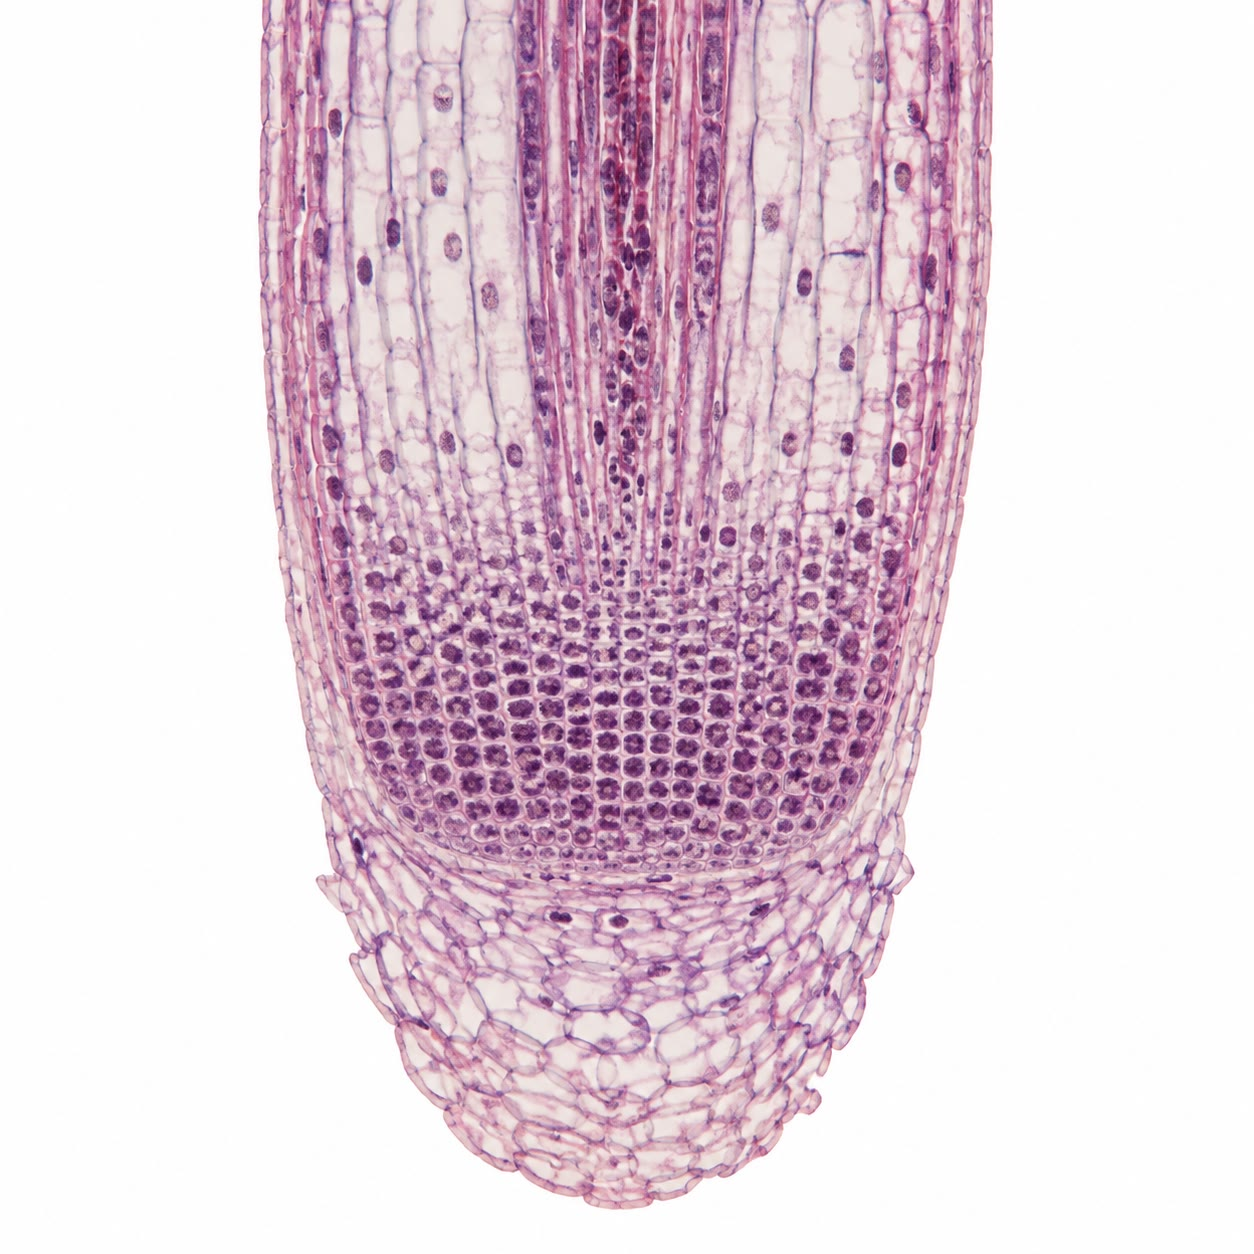
\includegraphics[width=0.42\linewidth]{images/book4/ai/b4-13-root-tip.jpg}

{\small طرف جذر في مقطع طولي: خلايا القلنسوة المفككة،
\omterm{def:b2:plant-meristems:meristem}{والمرستيم} الكثيف بنواه القاتمة، والخلايا المستطيلة
فوقه.}
\end{omfigure}

\section{كيف تنمو خلية نباتية}

\begin{theorem}[معادلة لوكهارت]\label{thm:b2:plant-meristems:lockhart}
\index{امتلاء}\index{جدار خلوي!قابلية التمدد}\index{معادلة لوكهارت}
تنمو الخلية النباتية بمط جدارها تحت ضغط
محتواها. ولا يستسلم الجدار استسلامًا لاعكوسًا إلا فوق عتبة من
الامتلاء $Y$، وعندها بمعدل يتناسب مع الفائض: فمعدل
النمو النسبي لخلية طولها $L$ هو
\[
\frac{1}{L}\frac{\mathrm{d}L}{\mathrm{d}t} = \phi\,(P - Y) \quad (P > Y),
\]
حيث $P$ ضغط الامتلاء و$\phi$ \emph{قابلية التمدد}
في الجدار. فالنمو مضبوط إذن من جهتين:
بالماء الذي يضبط $P$ (فالخلية الذابلة تكف عن النمو)، وبالجدار
الذي يضبط $\phi$ و$Y$ --- والجدار هو ما تعمل عليه
الهرمونات. فالأوكسين يجعل الخلايا تضخ البروتونات في الجدار؛
ويفعّل الحمض \emph{الإكسبانسينات}، وهي بروتينات ترخي الروابط بين
ليفيات السللوز والحشوة، فترفع $\phi$ وتخفض $Y$
في غضون دقائق (وهو \emph{النمو الحمضي}). فمع $\phi =
\qty{0.1}{h^{-1}.MPa^{-1}}$، و$Y = \qty{0.3}{MPa}$، و$P =
\qty{0.6}{MPa}$، تطول الخلية \qty{3}{\%} في الساعة وتتضاعف
في يوم؛ وفي منطقة استطالة جذر، حيث المعدلات أعلى بعدة
أضعاف، تطول الخلية عشرة أضعاف في ساعات قليلة.
\end{theorem}
\begin{proof}
الجدار مادة لزجة لدنة: فدون إجهاد الاستسلام
يتشوه مرنًا ويسترجع، وفوقه يجري بمعدل يتناسب
مع فائض الإجهاد. والإجهاد في الجدار يتناسب
مع ضغط الامتلاء (فمن أجل أسطوانة نصف قطرها $r$
وثخن جدارها $w$ يكون الإجهاد الطوقي $Pr/w$)، فيتناسب معدل
التشوه اللدن مع $P - Y$ بثابت $\phi$ يستوعب
الهندسة وخواص مادة الجدار. ومعدل التشوه
هو بالتعريف $(1/L)\,\mathrm{d}L/\mathrm{d}t$. وعدديًا،
$0.1\times(0.6 - 0.3) = \qty{0.03}{h^{-1}}$، ويتضاعف $L$ حين
$0.03\,t = \ln 2$، أي $t = \qty{23}{h}$.
\end{proof}

\begin{omfigure}
\begin{tikzpicture}
\begin{axis}[
  width=0.7\linewidth, height=5.4cm,
  axis x line=bottom, axis y line=left,
  xmin=0, xmax=1.0, ymin=0, ymax=0.09,
  xlabel={ضغط الامتلاء $P$ (\unit{MPa})}, ylabel={معدل النمو النسبي (\unit{h^{-1}})},
  xlabel style={font=\small, at={(axis description cs:0.5,-0.13)}, anchor=north},
  ylabel style={font=\small},
  tick label style={font=\small}, xtick={0,0.3,0.6,0.9}, ytick={0,0.03,0.06,0.09},
  yticklabels={0,0.03,0.06,0.09}, scaled y ticks=false,
  legend style={font=\scriptsize, at={(0.03,0.97)}, anchor=north west, draw=none},
  clip=false,
]
\addplot[very thick, omDef, domain=0:0.3, samples=2, forget plot] {0};
\addplot[very thick, omDef, domain=0.3:1.0, samples=2] {0.1*(x-0.3)};
\addlegendentry{$\phi = 0.1$، $Y = 0.3$}
\addplot[very thick, omThm, domain=0:0.2, samples=2, forget plot] {0};
\addplot[very thick, omThm, domain=0.2:0.65, samples=2] {0.2*(x-0.2)};
\addlegendentry{مع الأوكسين: $\phi = 0.2$، $Y = 0.2$}
\draw[dashed, gray] (axis cs:0.6,0) -- (axis cs:0.6,0.03); \node[font=\scriptsize, anchor=west] at (axis cs:0.61,0.015) {$P$ نموذجي};
\end{axis}
\end{tikzpicture}

{\small قانون لوكهارت: لا نمو دون امتلاء الاستسلام، ثم
معدل يتناسب مع الفائض. والأوكسين، بإرخائه الجدار،
يخفض العتبة ويزيد ميل المستقيم، فتنمو الخلية عند الامتلاء نفسه
أسرع بعدة أضعاف.}
\end{omfigure}

\begin{example}[من أين يأتي الماء]\label{ex:b2:plant-meristems:water}
بينما يستسلم الجدار، كان الامتلاء ليهبط ويتوقف النمو، لولا
دخول الماء ليجاري ذلك: فالخلية النامية تسرب وتعيد ملء نفسها.
والماء يأتي من \omterm{def:b2:plant-meristems:wood}{الخشب}، بتدرج صغير من كمون الماء،
ويضبط معدلَ دخوله ناقليةُ الغشاء المائية؛ فالنمو
أسرع ما يكون ليلًا، حين يقل النتح ويعلو الامتلاء، ويستطيع
ورق الذرة أن يمتد \qty{10}{cm} بين الغسق والفجر. وفي الجفاف تصنع
الخلايا منحلّات (\emph{التعديل التناضحي}) لتبقي $P$ فوق $Y$، وحين
يخفق ذلك تكف الورقة عن النمو قبل أيام من ذبولها.
\end{example}

\section{الهرمونات وشكل الفرع}

\begin{proposition}[الأوكسين والسيادة القمية]\label{prop:b2:plant-meristems:apical}
\index{أوكسين}\index{سيادة قمية}\index{نقل قطبي للأوكسين}\index{سيتوكينين}
\emph{الأوكسين} (حمض الإندول-3-أسيتيك) يُصنع في قمة الفرع
والأوراق الفتية ويُحمل نزولًا في الساق، خلية إلى خلية، بنحو
\qty{1}{cm/h}، بواسطة بروتينات ناقلة (PIN) مركّبة في الطرف السفلي
لكل خلية --- أي \emph{نقل قطبي} يعطي النبات
محورًا من الأعلى إلى الأسفل. وتيار الأوكسين النازل من القمة
يبقي البراعم الإبطية تحته ساكنة (\emph{\omterm{prop:b2:plant-meristems:apical}{السيادة القمية}})،
جزئيًا بمنعها من تصدير أوكسينها إلى
الساق، وجزئيًا باستحثاث الستريغولاكتونات وكبت السيتوكينين.
واقطع القمة تنمُ البراعم الأقرب إلى القطع في غضون أيام،
فيصير النبات كثيفًا --- وهو ما يستغله التقليم والتطويش.
و\emph{السيتوكينينات}، المصنوعة في أطراف الجذور والمحمولة صعودًا في \omterm{def:b2:plant-meristems:wood}{الخشب}،
تعزز نمو البراعم والانقسام الخلوي؛ و\emph{الجبريلينات}
تطيل السلاميات (فالبازلاء القزمة والقمح نصف القزم في
الثورة الخضراء معيبان في صنعها أو استشعارها)؛ وحمض
الأبسيسيك والإيثيلين يكبحان النمو تحت الإجهاد. فشكل الفرع ---
طويلًا أو كثيفًا، قائمًا أو منتشرًا --- مفاوضة بين
هذه الإشارات، ويضبط ميزانَ الجذر إلى الفرع الأوكسينُ
النازل في مقابل السيتوكينين الصاعد.
\end{proposition}
\begin{proof}[شواهد]
قطع ثيمان وسكوغ (1934) القمة من نباتات فاصولياء: فنمت البراعم
الجانبية. وكتلة من الآغار فيها أوكسين، موضوعة على الجذمور
المقطوع، أبقتها ساكنة كما كانت القمة؛ ولم يفعل الآغار وحده ذلك. وكان
فينت (1928) قد قاس الأوكسين بالانحناء الذي يحدثه في
غمد سويقة شوفان مقطوع الرأس حين يوضع على أحد جانبي الجذمور ---
وهو أول مقايسة حيوية لهرمون نباتي، وأصل الاسم،
من اليونانية بمعنى «أن ينمو». وقد بُيّنت قطبية النقل
بوضع آغار الأوكسين على أحد طرفي قطعة ساق وإيجاده
في كتلة مستقبِلة عند الطرف الآخر حين تكون القطعة
موجهة والقمة إلى الأعلى وحدها، مهما قُلبت القطعة في حقل
الجاذبية.
\end{proof}

\begin{omfigure}
\begin{tikzpicture}[every node/.style={font=\scriptsize}, >=stealth]
  \foreach \x/\lab/\apex/\aux in {0/{سليمة: القمة قائمة،\\والبراعم ساكنة}/1/0, 4.2/{مقطوعة الرأس:\\البراعم تنمو}/0/0, 8.4/{مقطوعة الرأس + أوكسين\\على الجذمور: ساكنة}/0/1} {
    \begin{scope}[xshift=\x cm]
      \draw[very thick, omExo!70!black] (0,0) -- (0,3.4);
      \foreach \y in {0.8,1.6,2.4} { \draw[thick, omExo!70!black] (0,\y) -- (-0.8,\y+0.4); \draw[thick, omExo!70!black] (0,\y+0.4) -- (0.8,\y+0.8); }
      \ifnum\apex=1 \draw[thick, fill=omThm!40] (0,3.5) ellipse (0.25 and 0.3); \draw[->, thick, omThm] (0.35,3.2) -- (0.35,1.0); \node[omThm, right] at (0.4,2.1) {أوكسين}; \fi
      \ifnum\apex=0 \draw[thick] (-0.3,3.4) -- (0.3,3.4); \fi
      \ifnum\aux=1 \draw[thick, fill=omThm!40] (-0.25,3.4) rectangle (0.25,3.75); \node[omThm, right] at (0.3,3.6) {آغار بالأوكسين}; \draw[->, thick, omThm] (0.35,3.2) -- (0.35,1.0); \fi
      \ifnum\apex=1 \foreach \y in {0.8,1.6,2.4} \fill[gray!60] (-0.12,\y+0.1) circle (0.08); \fi
      \ifnum\aux=1 \foreach \y in {0.8,1.6,2.4} \fill[gray!60] (-0.12,\y+0.1) circle (0.08); \fi
      \ifnum\apex=0 \ifnum\aux=0 \foreach \y in {0.8,1.6,2.4} { \draw[thick, omExo!70!black] (-0.1,\y+0.1) -- (-0.7,\y+0.9); \draw[thick, omExo!70!black] (-0.7,\y+0.9) -- (-1.0,\y+1.1); \draw[thick, omExo!70!black] (-0.7,\y+0.9) -- (-0.75,\y+1.25); } \fi\fi
      \node[below, align=center] at (0,-0.3) {\lab};
    \end{scope}
  }
\end{tikzpicture}

{\small \omterm{prop:b2:plant-meristems:apical}{السيادة القمية}، وتجربة ثيمان--سكوغ. القمة
تبقي البراعم الإبطية ساكنة؛ ونزعها يحررها؛ والأوكسين على
الجذمور المقطوع يحل محل القمة.}
\end{omfigure}

\begin{example}[إشارة سريعة، وجزيئة بطيئة]\label{ex:b2:plant-meristems:transport}
ينقل النقل القطبي الأوكسين \qty{1}{cm} في ساعة؛ أما الانتشار وحده
فكان ليستغرق، للسنتيمتر نفسه، $t = x^2/2D = 10^{-4}/(2\times
10^{-9}) = \qty{5e4}{s}$ --- أي أربع عشرة ساعة --- وللعشرة
سنتيمترات إلى برعم أسفل، ستين يومًا. فالضخ والترحيل في
ناقلات PIN هما ما يجعل إشارة هرمونية صالحة للاستعمال على طول
نبات؛ والناقلات نفسها، منقولةً إلى الجانب المظلل من ساق،
تحنيها نحو الضوء (\cref{ch:b2:plant-plasticity}).
\end{example}

\section{النمو الثانوي: الخشب والقلف}

\begin{definition}[الكامبيوم الوعائي والخشب]\label{def:b2:plant-meristems:wood}
\index{كامبيوم وعائي}\index{خشب}\index{حلقة سنوية}\index{قلف}\index{بريدرم}
في الساق الخشبية تُوصل خصل الخشب واللحاء الأوليين،
في السنة الأولى، في أسطوانة متصلة من خلايا منقسمة، هي
\emph{\omterm{def:b2:plant-meristems:meristem}{الكامبيوم} الوعائي}. وتنقسم خلاياه مماسيًا، فتضيف
\emph{خشبًا ثانويًا} --- أي \emph{الخشب} --- إلى الداخل و
\emph{لحاءً ثانويًا} إلى الخارج، فيتحرك \omterm{def:b2:plant-meristems:meristem}{الكامبيوم}
خارجًا مع تثخن الجذع، ويضيف انقسامات شعاعية عارضة
لتوسيع الحلقة. وفي المناخات الموسمية يكون الخشب الموضوع
في الربيع ذا أوعية واسعة رقيقة الجدر (\emph{الخشب الباكر}) وخشب
الصيف ذا أوعية ضيقة سميكة الجدر (\emph{الخشب المتأخر})، فتترك كل
سنة \emph{حلقة سنوية} مرئية؛ وتسجل الحلقات
عمر الشجرة، وتسجل بعروضها مناخ كل سنة
(وهو علم تأريخ الحلقات). ولا يوصّل إلا الحلقات الخارجية، أي \emph{الخشب
العصاري}؛ أما الداخلية، أي \emph{الخشب القلبي}، فميتة مسدودة
ومقتمة بالراتنجات والعفصيات، وتخدم هيكلًا
للشجرة. وخارج اللحاء يصنع \omterm{def:b2:plant-meristems:meristem}{مرستيم} جانبي ثانٍ، هو
\emph{\omterm{def:b2:plant-meristems:meristem}{كامبيوم} الفلين}، \emph{البريدرم} --- أي طبقات من خلايا فلينية
ميتة مقاومة للماء بالسوبرين --- وهو مع اللحاء القديم
\emph{القلف}. فالجذع إذن قشرة حية رقيقة من
\omterm{def:b2:plant-meristems:meristem}{كامبيوم} وخشب عصاري ولحاء حول لبّ ميت، تحت جلد ميت.
\end{definition}

\begin{omfigure}
\begin{tikzpicture}[every node/.style={font=\scriptsize}]
  \fill[omExo!60] (0,0) circle (3.0);
  \fill[omDef!20] (0,0) circle (2.75);
  \fill[omDef!35] (0,0) circle (2.2);
  \foreach \r in {0.4,0.7,1.0,1.3,1.6,1.9,2.2} \draw[omDef!80!black, thin] (0,0) circle (\r);
  \fill[omExo!80!black] (0,0) circle (1.3);
  \foreach \r in {0.4,0.7,1.0} \draw[omExo!40, thin] (0,0) circle (\r);
  \draw[very thick, omThm] (0,0) circle (2.5);
  \draw (2.9,0.6) -- (3.9,1.6) node[right, align=left] {القلف: فلين (بريدرم)\\ولحاء قديم};
  \draw (2.62,0.0) -- (3.9,0.6) node[right] {لحاء ثانوي، حي};
  \draw (2.5,-0.4) -- (3.9,-0.4) node[right] {كامبيوم وعائي (بالأحمر)};
  \draw (1.9,-1.1) -- (3.9,-1.4) node[right, align=left] {خشب عصاري: حلقات حديثة،\\موصّلة};
  \draw (0.5,-0.9) -- (3.9,-2.4) node[right, align=left] {خشب قلبي: حلقات قديمة،\\ميتة مسدودة};
  \draw (-1.7,1.5) -- (-3.6,2.4) node[left, align=right] {حلقة سنوية واحدة:\\خشب باكر فاتح،\\وخشب متأخر قاتم};
\end{tikzpicture}

{\small جذع في مقطع عرضي. يضيف \omterm{def:b2:plant-meristems:meristem}{الكامبيوم} (بالأحمر) خشبًا إلى الداخل
ولحاءً إلى الخارج كل سنة؛ والحلقات الحديثة توصّل، والقديمة
تكوّن \omterm{def:b2:plant-meristems:wood}{الخشب} القلبي الميت؛ والفلين واللحاء القديم يصنعان \omterm{def:b2:plant-meristems:wood}{القلف}.}
\end{omfigure}

\begin{theorem}[لماذا تضيف شجرة عتيقة خشبًا أكثر]\label{thm:b2:plant-meristems:rings}
جذع نصف قطره $r$ وارتفاعه $h$ يضيف كامبيومه حلقة
ثخنها $\Delta r$ كل سنة يكسب حجمًا من \omterm{def:b2:plant-meristems:wood}{الخشب}
\[
\Delta V \approx 2\pi r\,h\,\Delta r
\]
في السنة: فعند عرض حلقة ثابت، تنمو الزيادة السنوية
بنسبة نصف القطر، وشجرة نصف قطرها \qty{50}{cm} تضيف عشرة
أضعاف \omterm{def:b2:plant-meristems:wood}{خشب} شجرة نصف قطرها \qty{5}{cm}، وإن لم تكن حلقاتها
أعرض. وجذع نصف قطره \qty{25}{cm} وارتفاعه \qty{10}{m} يضيف
\qty{4}{mm} في السنة يكسب \qty{0.063}{m^3}، أي نحو \qty{30}{kg} من
\omterm{def:b2:plant-meristems:wood}{الخشب} الجاف --- أي \qty{15}{kg} من الكربون، سحبه التاج من الهواء في
موسم واحد.
\end{theorem}
\begin{proof}
\omterm{def:b2:plant-meristems:wood}{الخشب} المضاف قشرة أسطوانية محيطها $2\pi r$،
وثخنها $\Delta r$ وارتفاعها $h$؛ وحجمها $2\pi r h\Delta r$
إلى الرتبة الأولى في $\Delta r$ (وبالضبط $\pi h[(r + \Delta r)^2 - r^2]
= \pi h(2r\Delta r + \Delta r^2)$). فمع $r = 0.25$، و$h = 10$، و
$\Delta r = 0.004$: $2\pi\times 0.25\times 10\times 0.004 =
\qty{0.063}{m^3}$؛ وعند \qty{500}{kg/m^3} جافًا، \qty{31}{kg}، نصفها
كربون.
\end{proof}

\begin{omfigure}
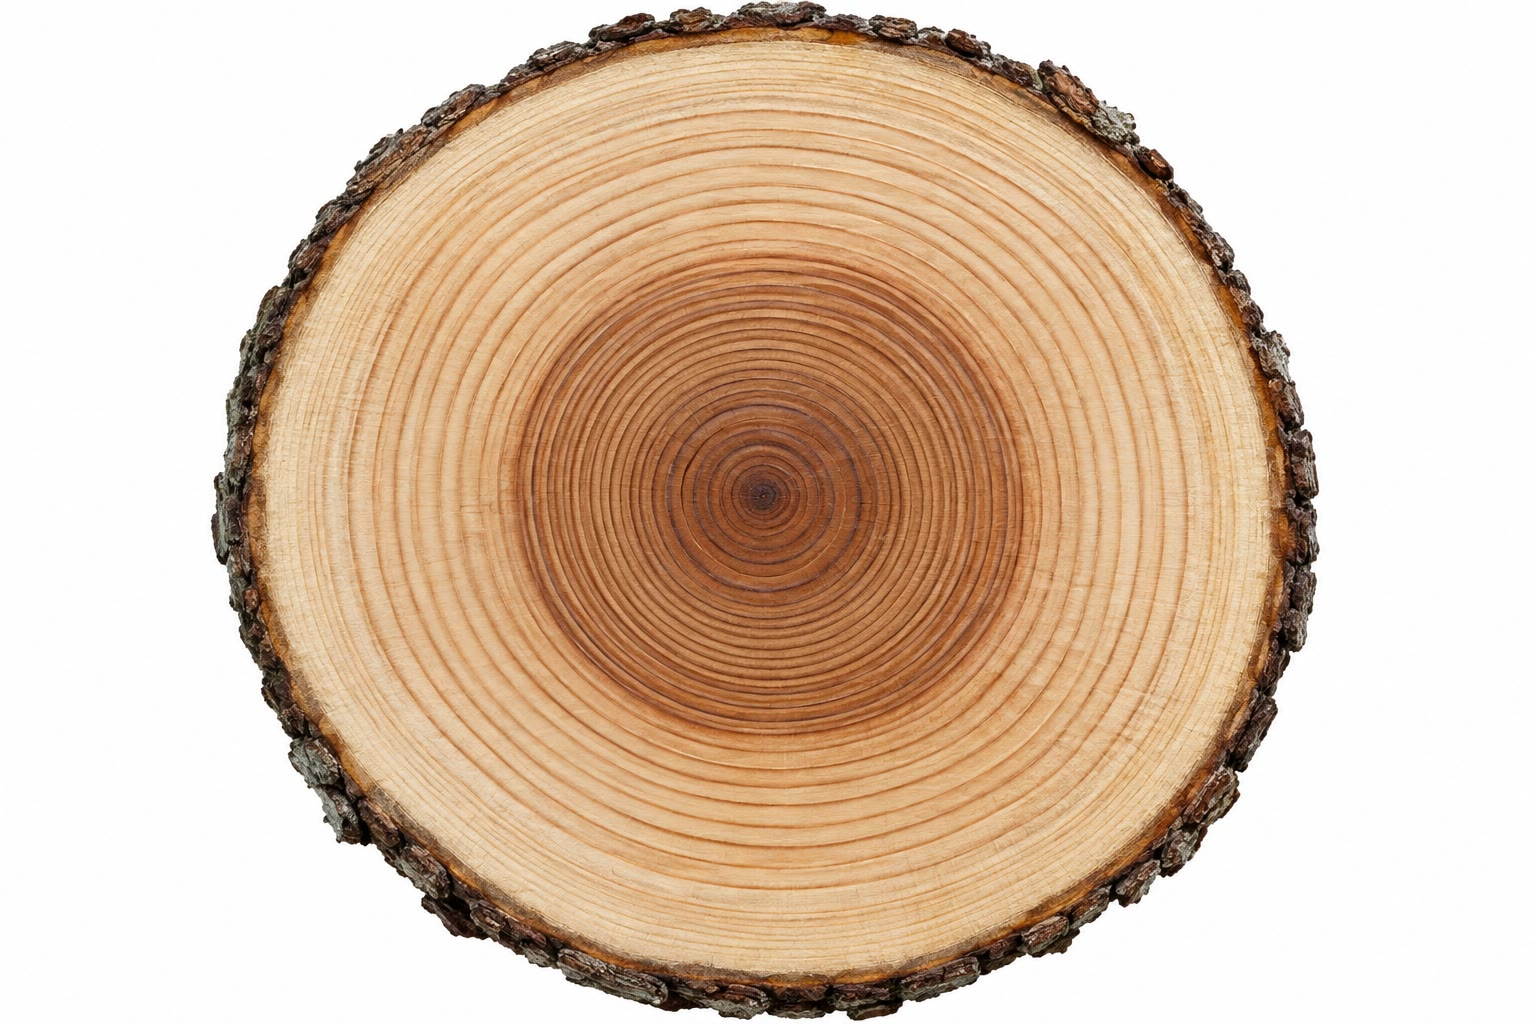
\includegraphics[width=0.5\linewidth]{images/book4/ai/b4-13-wood-rings.jpg}

{\small جذع صنوبر في مقطع عرضي: الحلقات السنوية، كل منها شريط
فاتح من \omterm{def:b2:plant-meristems:wood}{الخشب} الباكر وشريط قاتم من \omterm{def:b2:plant-meristems:wood}{الخشب} المتأخر، \omterm{def:b2:plant-meristems:wood}{والخشب} القلبي الأقتم،
\omterm{def:b2:plant-meristems:wood}{والقلف}.}
\end{omfigure}

\section{تمارين}

\begin{exercise}[$\star$]\label{exo:b2:plant-meristems:1}
عرّف \omterm{def:b2:plant-meristems:meristem}{المرستيم}، وسمِّ مرستيمات نبات خشبي الأربعة مع
ما ينتجه كل منها.
\end{exercise}

\begin{exercise}[$\star$]\label{exo:b2:plant-meristems:2}
اذكر مناطق طرف الجذر من القلنسوة صاعدًا، مع ما يحدث
لخلية في كل منها. ومن أين تأتي الجذور الجانبية؟
\end{exercise}

\begin{exercise}[$\star$]\label{exo:b2:plant-meristems:3}
صف تجربة ثيمان--سكوغ وشاهدها و
استنتاجها.
\end{exercise}

\begin{exercise}[$\star$]\label{exo:b2:plant-meristems:4}
مقطع جذع يُظهر 60 حلقة، الخارجية منها 15 فاتحة والبقية قاتمة.
أعط عمر الشجرة، وعمر خشبها العصاري، وقل أي جزء
من الجذع حي.
\end{exercise}

\begin{exercise}[$\star\star$]\label{exo:b2:plant-meristems:5}
مع $\phi = \qty{0.1}{h^{-1}.MPa^{-1}}$، و$Y = \qty{0.3}{MPa}$، احسب
معدل النمو النسبي عند $P = 0.4$ و$0.6$ و\qty{0.8}{MPa}، و
زمن التضاعف عند كل منها. وجفاف يخفض $P$ إلى \qty{0.25}{MPa}:
فماذا يحدث؟
\end{exercise}

\begin{exercise}[$\star\star$]\label{exo:b2:plant-meristems:6}
تنشأ الأوراق المتعاقبة على \qty{137.5}{\degree} بعضها من بعض.
احسب المواضع الزاوية للأوراق 1 إلى 8 (بترديد
\qty{360}{\degree}) وبيّن أن لا ورقتين من الثماني الأولى تقعان
ضمن \qty{20}{\degree} إحداهما من الأخرى. ولماذا يهم هذا
النبات؟
\end{exercise}

\begin{exercise}[$\star\star$]\label{exo:b2:plant-meristems:7}
شجرة طولها \qty{12}{m} تضيف حلقات من \qty{3}{mm}. احسب \omterm{def:b2:plant-meristems:wood}{الخشب}
المضاف في السنة التي يكون فيها نصف قطرها \qty{5}{cm} وفي السنة التي يكون فيها
\qty{40}{cm}، والكربون المقابل (الكثافة الجافة
\qty{500}{kg/m^3}، ونصفها كربون).
\end{exercise}

\begin{exercise}[$\star\star$]\label{exo:b2:plant-meristems:8}
تنبّأ بالأنماط الظاهرية لطافرة \emph{clv3} وطافرة \emph{wus}
والطافرة المضاعفة، واشرح ترتيب المورّثتين في
الحلقة انطلاقًا من الطافرة المضاعفة.
\end{exercise}

\begin{exercise}[$\star\star$]\label{exo:b2:plant-meristems:9}
يُنقل الأوكسين بسرعة \qty{1}{cm/h}؛ ومعامل انتشاره في
النسيج \qty{1e-9}{m^2/s}. فكم تستغرق الإشارة لتبلغ
برعمًا يبعد \qty{20}{cm} تحت القمة بالنقل، وبالانتشار
($t = x^2/2D$)؟ وماذا يشتري النقل القطبي للنبات؟
\end{exercise}

\begin{exercise}[$\star\star\star$]\label{exo:b2:plant-meristems:10}
ينمو جذر ذرة \qty{3}{cm} في اليوم. وخلايا \omterm{def:b2:plant-meristems:meristem}{المرستيم} طولها
\qty{20}{\micro m} وتستطيل عشرة أضعاف قبل أن تنضج؛ وفي كل
رتل خلوي نحو \num{100} خلية منقسمة. فكم خلية يجب أن ينتج
\omterm{def:b2:plant-meristems:meristem}{مرستيم} كل رتل في اليوم، وأي زمن دورة خلوية
يستلزم ذلك؟
\end{exercise}

\begin{exercise}[$\star\star\star$]\label{exo:b2:plant-meristems:11}
أقماح الستينيات نصف القزمة تحمل طفرات تجعل
النبات عديم الحساسية للجبريلين. اشرح لماذا تكون قصيرة، ولماذا
يستطيع نبات قصير أن يعطي حبًا أكثر حين يُسمَّد بغزارة، ولماذا
تكون \omterm{def:b2:genome-diversification:mutation}{الطفرة} نفسها في نبات بري مساوئ.
\end{exercise}

\begin{exercise}[$\star\star\star$]\label{exo:b2:plant-meristems:12}
«الحيوان يُبنى مرة؛ والنبات يُبنى طوال حياته.» ناقش
عواقب النمو المرستيمي على قدرة النبات على
الاستجابة لمحيطه، وعلى النجاة من الأذى، وعلى العيش
آلاف السنين --- وكلفةً واحدة للاستراتيجية.
\end{exercise}

\section{مسألة: شجرة بالأرقام}

\begin{problem}[{مسألة نهاية الأسبوع --- متابعة شجرة فتية سنةً:
الأوراق التي تصنعها قمتها، ونمو سلامية بقانون لوكهارت،
والخشب الذي يضعه كامبيومها والكربون الذي يكلفه، و
استجابة براعمها للتقليم، وتنتهي إلى الأوراق في السنة،
ونمو السلامية في الساعة، وخشب السنة}]
\label{pb:b2:plant-meristems:1}
لشجرة زيزفون فتية \num{200} طرف فرع نامٍ؛ وتبدئ كل قمة
ورقة كل \num{3} أيام خلال موسم من \num{150} يومًا، على
فترات \qty{137.5}{\degree}. والسلامية النامية طولها \qty{2}{cm}،
ولخلاياها $\phi = \qty{0.05}{h^{-1}.MPa^{-1}}$، و$Y =
\qty{0.35}{MPa}$؛ والامتلاء \qty{0.55}{MPa} نهارًا و
\qty{0.75}{MPa} ليلًا (\qty{12}{h} لكل منهما). والجذع
طوله \qty{8}{m} ونصف قطره \qty{10}{cm}؛ ويضيف \omterm{def:b2:plant-meristems:meristem}{الكامبيوم}
\qty{5}{mm} في السنة؛ \omterm{def:b2:plant-meristems:wood}{والخشب} الجاف \qty{500}{kg/m^3} ونصفه كربون.
ويحمل التاج \qty{80}{m^2} من الأوراق تثبّت صافيًا \qty{4}{g} من
الكربون في المتر المربع في اليوم مدة \num{150} يومًا.

\medskip
\noindent\textbf{الجزء الأول --- الأوراق.}
\begin{enumerate}
  \item كم ورقة تصنع قمة واحدة في الموسم؟ والشجرة
        كلها؟
  \item احسب المواضع الزاوية للأوراق 1 إلى 5 على فرع واحد.
  \item بعد كم ورقة تقع ورقة ضمن
        \qty{10}{\degree} من الورقة 1؟ (جرّب مضاعفات
        \qty{137.5}{\degree}.)
  \item ماذا تحقق الزاوية الذهبية للنبات، وأي هرمون
        ينتج نقله إياها؟
  \item إذا كانت مساحة كل ورقة \qty{80}{cm^2}، فأي مساحة أوراق
        تبنيها الشجرة في الموسم؟ وقارنها بمساحة \qty{80}{m^2}
        التي تحملها في منتصف الصيف.
  \item الشجرة نفضية. فأي كسر من مساحة أوراقها تعيد بناءه
        كل ربيع، ومن أين يأتي كربون الأوراق الأولى؟
  \item \omterm{def:b2:genome-diversification:mutation}{طفرة} \emph{clv3} تثلّث قياس كل قمة. فما الذي
        يتغير في جوابي السؤالين 1 و5، وكيف تبدو
        الفروع؟
\end{enumerate}

\medskip
\noindent\textbf{الجزء الثاني --- سلامية.}
\begin{enumerate}[resume]
  \item احسب معدل النمو النسبي نهارًا وليلًا.
  \item احسب الطول المضاف في نهار واحد وليل واحد، انطلاقًا
        من \qty{2}{cm}.
  \item وعلى مدى أربعة أيام كهذه، ما طول السلامية؟
        (عامل النمو تراكميًا، $L(t) = L_0 e^{rt}$ بالمعدل
        المتوسط.)
  \item معالجة بالجبريلين تخفض $Y$ إلى \qty{0.25}{MPa}.
        أعد حساب معدلي النهار والليل.
  \item جفاف يبقي الامتلاء عند \qty{0.4}{MPa} ليلًا ونهارًا.
        احسب المعدل، وقل ماذا يفعل التعديل التناضحي.
  \item اشرح لماذا يفوق نمو الليل نمو النهار مع أن
        التركيب الضوئي يقع نهارًا.
\end{enumerate}

\medskip
\noindent\textbf{الجزء الثالث --- \omterm{def:b2:plant-meristems:wood}{الخشب}.}
\begin{enumerate}[resume]
  \item احسب حجم \omterm{def:b2:plant-meristems:wood}{الخشب} المضاف هذه السنة وكتلته الجافة.
  \item احسب الكربون فيه.
  \item احسب الكربون الذي يثبّته التاج على مدى الموسم.
  \item ما كسر كربون التاج الذي ذهب إلى \omterm{def:b2:plant-meristems:wood}{خشب} الجذع؟
        وسمِّ ثلاثة مصارف أخرى.
  \item بعد عشرين سنة، وبعرض الحلقة نفسه، أي زيادة \omterm{def:b2:plant-meristems:wood}{خشب}
        سنوية تكون؟ ولماذا ترتفع؟
  \item حلقتان من الجذع نصف عرض جاراتهما.
        اقترح سببين وكيف يميّز بينهما مؤرخ
        الحلقات.
\end{enumerate}

\medskip
\noindent\textbf{الجزء الرابع --- البراعم والتقليم.}
\begin{enumerate}[resume]
  \item يقصّ البستاني كل طرف فرع. تنبّأ باستجابة
        البراعم الإبطية وبشكل الشجرة بعد شهر.
  \item كيف يغير معجون أوكسين على كل قطع الاستجابة؟
  \item يُقلَّم سياج ست مرات في السنة. اشرح، \omterm{prop:b2:plant-meristems:apical}{بالسيادة
        القمية}، لماذا يصير كثيفًا.
  \item شجرة قُطعت إلى جذمور تنمي عشرات الفروع. فمن أين
        تأتي، ولماذا يستطيع النبات النجاة من فقد كل
        فرع بينما لا يستطيع الحيوان النجاة من فقد رأسه؟
  \item يرتفع السيتوكينين من الجذور بعد ريّها.
        تنبّأ بالأثر في نمو البراعم.
  \item اذكر النتيجة: الأوراق في القمة وفي الشجرة في الموسم،
        ومعدلا نمو السلامية نهارًا وليلًا، \omterm{def:b2:plant-meristems:wood}{وخشب} السنة وكربونها.
\end{enumerate}
\end{problem}
